\ylDisplay{Läätsede süsteem} % Ülesande nimi
{EFO žürii} % Autor
{piirkonnavoor} % Voor
{2017} % Aasta
{P 4} % Ülesande nr.
{2} % Raskustase
{
% Teema: Valgusõpetus
\ifStatement
Kaks läätse optiliste tugevustega $D_1 = 10$ $dpt$ ja $D_2 = 5$ $dpt$ asuvad teineteisest $60$ $cm$ kaugusel. Läätsede optilised peateljed ühtivad. Ese asub esimese läätse ees, sellest $20$ $cm$ kaugusel optilisel peateljel. Kui kaugele teise läätse taha tekib optilise süsteemi poolt tekitatud kujutis, kui suur see on võrreldes esemega ning kas see on ümberpööratud või päripidine? 
\begin{center}
	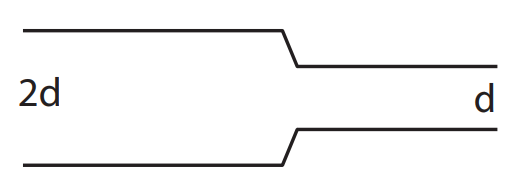
\includegraphics[width=0.5\linewidth]{2017-v2p-04-yl.PNG}
\end{center}
\fi
\ifHint
Optiliste tugevuste põhjal on võimalik arvutada läätsede fookuskaugused. Tuleb mõista, et kui ese asub kahe fookuskauguse kaugusel läätsest, asub ka selle kujutis kahe fookuskauguse kaugusel läätsest, on ümberpööratud ja eseme suurune.
\fi
\ifSolution
Valemist $f = \frac{1}{D}$ selgub, et esimese läätse fookuskaugus on $10$ cm ja teise läätse fookuskaugus $20$ cm. Kuivõrd ese asub esimesest läätsest $20$ cm kaugusel, asub ese täpselt $2$ fookuskauguse kaugusel läätsest. Kui ese asub kahe fookuskauguse kaugusel läätsest, asub ka selle kujutis kahe fookuskauguse kaugusel läätsest, on ümberpööratud ja eseme suurune. Kuna läätsede kaugus teineteisest on $60$ cm, asub esimese läätse poolt tekitatud eseme kujutis teisest läätsest täpselt kahe fookuskauguse kaugusel. Seega tekitab läätsede süsteem kujutise, mis asub teisest läätsest $40$ cm kaugusel, on eseme suurune ja esemega võrreldes päripidine.
\fi
}
